\subsection{Holography}
\label{sec.holography}



%While the terms holography and hologram are used without distinction in many works in the literature, this work defines holography the imprint of the light in a film and hologram the reproduction of the holography. This is made to create a distinction between the process of recording and reproduction.  Moreover, it make an etymological coherence with photography --- which is recorded in a film --- and photogram --- the photographic image made without a camera by placing objects directly onto the surface of a light-sensitive material. Some of the earliest photographic works ever made are photograms. The charm of this technique, requiring no camera or lens, comes from light shone onto photographic paper or film with objects in the way, casting deep and translucent shadows, as illustrated in Figure~\ref{fig:photogram}.

%\begin{figure}[!ht]
%\centering
%\includegraphics[width=0.9\linewidth,keepaspectratio=true]{figs/photog%ram.jpg}
%\caption{Photogram. ©Aberlado Morell}
%\label{fig:photogram}
%\end{figure}



%While a photograph can be made using unorganized white light, the holography needs organized light of a laser is necessary because to recording the differences in both amplitude and the phase. In order for the film to record these differences, all the waves have to be identical when they leave the laser, as show in Figure~\ref{fig.hologram}a. The holographic film records very small changes in light and can be a emulsion that respond most strongly to red light.

%When a column of light leaves the laser and passes through the beam splitter, the two columns reflect off of their respective mirrors and pass through their respective diverging lenses, as shown in Figure~\ref{fig.hologram}b.The object reflects off of the object and combines with the reference beam at the holographic film.

%Some portion of light that reach the surface of the object is absorbed and the rest is reflected diffusely in the rough microscopic surface, even if it looks smooth to the human eye. It scatters light in every direction following the Fresnel's law of reflection: the angle of incidence is the same as its angle of reflection. The light reflected from every part of the object travels to reach every part of the holographic plate, and therefore, it captures information about each portion of the object.

%In summary, the tools needed to make a hologram are:

%\begin{itemize}
%\item A coherent light beam, usually helium-neon (HeNe) red lasers, which are common source of coherent light in holography. Some types of holograms use lasers with different wavelengths that produce different colors of light, and, depending on the type of laser you're using, you may also need a shutter to control the exposure.

%\item Lenses, used to spread out the beam of light.

%\item A beam splitter, which can be mirrors and prisms, used to split one beam of light into two beams.

%\item Mirrors, to direct the beams of light to the correct locations. Along with the lenses and beam splitter, the mirrors have to be absolutely clean.

%\item A holographic film, that records light at a very high resolution, which is necessary for creating a holography. It's a layer of light-sensitive compounds on a transparent surface, like photographic film. The difference between holographic and photographic film is that holographic film has to be able to record very small changes in light that take place over microscopic distances. In other words, it needs to have a very fine grain. In some cases, holograms that use a red laser rely on emulsions that respond most strongly to red light.
 
%\end{itemize}
%The tools needed to make a hologram are: red lasers, lenses, mirrors and a holographic film. There are many ways to arrange these tools. In the basic transmission hologram setup the laser points at the beam splitter, which divides the beam of light into two parts.

%Mirrors direct the paths of these two beams so that they hit their intended targets. Each of the two beams passes through a diverging lens and becomes a wide swath of light rather than a narrow beam. One beam, the object beam, reflects off of the object and onto the photographic emulsion. The other beam, the reference beam, hits the emulsion without reflecting off of anything other than a mirror.

%The microscopic interference fringes on a hologram are both dark and microscopic, that changes the monochrome light when it passes through it. It produces a 3D image in the same spot where the object was when the hologram was made. First, the light passes through a diverging lens, which causes monochromatic light -- or light that consists of one wavelength color -- to hit every part of the hologram simultaneously. Since the hologram is transparent, it transmits most of the light, which passes through unchanged as show in Figure~\ref{fig.hologram}c.


%The interference fringes reflect some of the light, acting as a curved, microscopic mirror. Light that hits it follows the Fresnel law of reflection  and its angle of incidence equals its angle of reflection, deflecting it in different directions. The scattered light beams create an image in the process.

%This process is a direct result of the light traveling as a wave -- when a wave moves past an obstacle or through a slit, its wave front expands on the other side. There are so many slits among the interference fringes of a hologram that it acts like a diffraction grating, causing lots of intersecting wave fronts to appear in a very small space, as shown in Figure~\ref{fig.hologram}d.

\begin{figure}
\centering
\begin{tabular}{cc}
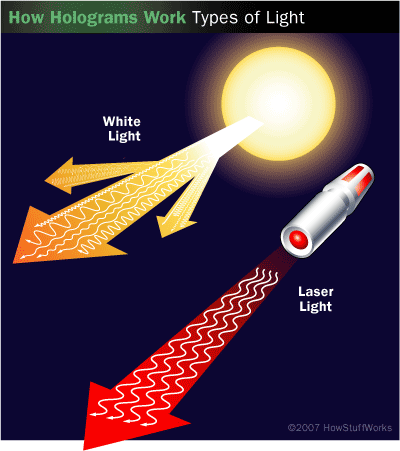
\includegraphics[width=0.45\linewidth,keepaspectratio=true]{figs/hologram01.png}&
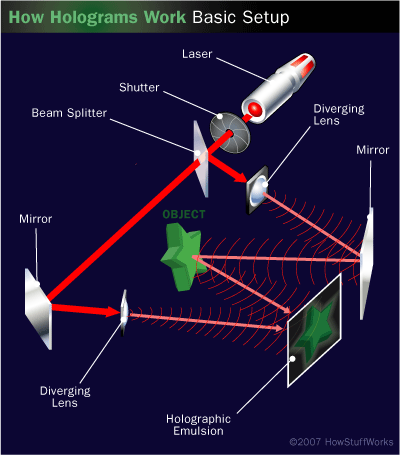
\includegraphics[width=0.45\linewidth,keepaspectratio=true]{figs/hologram02.png}\\
(a)&(b)\\
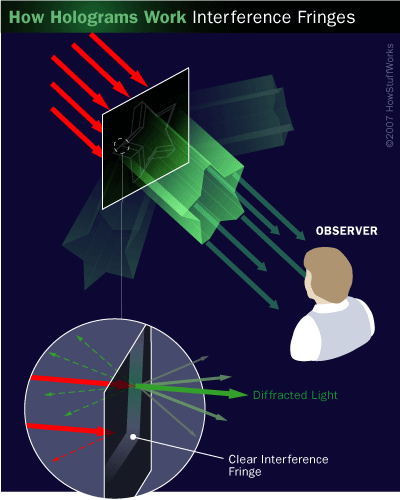
\includegraphics[width=0.45\linewidth,keepaspectratio=true]{figs/hologram03.png}&
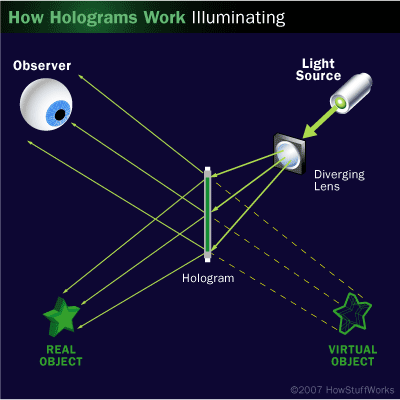
\includegraphics[width=0.45\linewidth,keepaspectratio=true]{figs/hologram04.png}\\ 
(c)&(d)\\
\end{tabular}
\caption{How hologram works. ©HowStuffWorks}
\label{fig.hologram}
\end{figure}